%%%%%%%%%%%%%%%%%%%%%%%%%%%%%%%%%%%%%%%%%%%%%%%%%%%%%%%%%%%%%%%%%%%%%%
%%  disstemplate.tex, to be compiled with latex.             %
%%  08 April 2002   Version 4                    %
%%%%%%%%%%%%%%%%%%%%%%%%%%%%%%%%%%%%%%%%%%%%%%%%%%%%%%%%%%%%%%%%%%%%%%
%%                                   %
%%  Writing a Doctoral Dissertation with LaTeX at            %
%%  the University of Texas at Austin                %
%%                                   %
%%  (Modify this ``template'' for your own dissertation.)        %
%%                                   %
%%%%%%%%%%%%%%%%%%%%%%%%%%%%%%%%%%%%%%%%%%%%%%%%%%%%%%%%%%%%%%%%%%%%%%


\documentclass[12pt]{report}    % The documentclass must be ``report''.

\usepackage{utdiss2}        % Dissertation package style file.


%%%%%%%%%%%%%%%%%%%%%%%%%%%%%%%%%%%%%%%%%%%%%%%%%%%%%%%%%%%%%%%%%%%%%%
% Optional packages used for this sample dissertation. If you don't  %
% need a capability in your dissertation, feel free to comment out   %
% the package usage command.                         %
%%%%%%%%%%%%%%%%%%%%%%%%%%%%%%%%%%%%%%%%%%%%%%%%%%%%%%%%%%%%%%%%%%%%%%

\usepackage{amsmath,amsthm,amsfonts,amscd}
                % Some packages to write mathematics.
\usepackage{eucal}      % Euler fonts
\usepackage{verbatim}       % Allows quoting source with commands.
\usepackage{makeidx}        % Package to make an index.
\usepackage{psfig}          % Allows inclusion of eps files.
\usepackage{epsfig}             % Allows inclusion of eps files.
\usepackage{citesort}           %
\usepackage{url}        % Allows good typesetting of web URLs.
\usepackage{draftcopy}     % Uncomment this line to have the
                % word, "DRAFT," as a background
                % "watermark" on all of the pages of
                % of your draft versions. When ready
                % to generate your final copy, re-comment
                % it out with a percent sign to remove
                % the word draft before you re-run
                % Makediss for the last time.

\author{Alexander Dean}    % Required

\address{670 Westchester Rd. \\ Grosse Pointe, Michigan 48230}  % Required

\title{Process Cooperativity as a Feedback Metric \\
                in Concurrent Message-Passing Languages}
                                                    % Required

%%%%%%%%%%%%%%%%%%%%%%%%%%%%%%%%%%%%%%%%%%%%%%%%%%%%%%%%%%%%%%%%%%%%%%
% NOTICE: The total number of supervisors and other members %%%%%%%%%%
%%%%%%%%%%%%%%% MUST be seven (7) or less! If you put in more, %%%%%%%
%%%%%%%%%%%%%%% they are put on the page after the Committee %%%%%%%%%
%%%%%%%%%%%%%%% Certification of Approved Version page. %%%%%%%%%%%%%%
%%%%%%%%%%%%%%%%%%%%%%%%%%%%%%%%%%%%%%%%%%%%%%%%%%%%%%%%%%%%%%%%%%%%%%

%%%%%%%%%%%%%%%%%%%%%%%%%%%%%%%%%%%%%%%%%%%%%%%%%%%%%%%%%%%%%%%%%%%%%%
%
% Enter names of the supervisor and co-supervisor(s), if any,
% of your dissertation committee. Put one name per line with
% the name in square brackets. The name on the last line, however,
% must be in curly braces.
%
% If you have only one supervisor, the entry below will read:
%
%   \supervisor
%       {Supervisor's Name}
%
% NOTE: Maximum three supervisors. Minimum one supervisor.
% NOTE: The Office of Graduate Studies will accept only two supervisors!
%
%
\supervisor
    {Dr. Matthew Fluet}

%%%%%%%%%%%%%%%%%%%%%%%%%%%%%%%%%%%%%%%%%%%%%%%%%%%%%%%%%%%%%%%%%%%%%%
%
% Enter names of the other (non-supervisor) members(s) of your
% dissertation committee. Put one name per line with the name
% in square brackets. The name on the last line, however, must
% be in curly braces.
%
% NOTE: Maximum six other members. Minimum zero other members.
% NOTE: The Office of Graduate Studies may restrict you to a total
%   of six committee members.
%
%
\committeemembers
%    [Erwin Schr\"odinger]
    [Dr. James Heliotis, Reader]
    {Dr. Rajendra K. Raj, Observer}
%    {Arthur Schawlow}

%%%%%%%%%%%%%%%%%%%%%%%%%%%%%%%%%%%%%%%%%%%%%%%%%%%%%%%%%%%%%%%%%%%%%%

\previousdegrees{B.S.}
     % The abbreviated form of your previous degree(s).
     % E.g., \previousdegrees{B.S., MBA}.
     %
     % The default value is `B.S., M.S.'

%\graduationmonth{...}
     % Graduation month, either May, August, or December, in the form
     % as `\graduationmonth{May}'. Do not abbreviate.
     %
     % The default value (either May, August, or December) is guessed
     % according to the time of running LaTeX.

%\graduationyear{...}
     % Graduation year, in the form as `\graduationyear{2001}'.
     % Use a 4 digit (not a 2 digit) number.
     %
     % The default value is guessed according to the time of
     % running LaTeX.

%\typist{...}
     % The name(s) of typist(s), put `the author' if you do it yourself.
     % E.g., `\typist{Maryann Hersey and the author}'.
     %
     % The default value is `the author'.


%%%%%%%%%%%%%%%%%%%%%%%%%%%%%%%%%%%%%%%%%%%%%%%%%%%%%%%%%%%%%%%%%%%%%%
% Commands for master's theses and reports.              %
%%%%%%%%%%%%%%%%%%%%%%%%%%%%%%%%%%%%%%%%%%%%%%%%%%%%%%%%%%%%%%%%%%%%%%
%
% If the degree you're seeking is NOT Doctor of Philosophy, uncomment
% (remove the % in front of) the following two command lines (the ones
% that have the \ as their second character).
%
\degree{Master of Science} \degreeabbr{M.S.}

% Uncomment the line below that corresponds to the type of master's
% document you are writing.
%
%\masterreport
\masterthesis


%%%%%%%%%%%%%%%%%%%%%%%%%%%%%%%%%%%%%%%%%%%%%%%%%%%%%%%%%%%%%%%%%%%%%%
% Some optional commands to change the document's defaults.      %
%%%%%%%%%%%%%%%%%%%%%%%%%%%%%%%%%%%%%%%%%%%%%%%%%%%%%%%%%%%%%%%%%%%%%%
%
\singlespacing
%\oneandonehalfspacing

%\singlespacequote
\oneandonehalfspacequote

\topmargin 0.125in  % Adjust this value if the PostScript file output
            % of your dissertation has incorrect top and
            % bottom margins. Print a copy of at least one
            % full page of your dissertation (not the first
            % page of a chapter) and measure the top and
            % bottom margins with a ruler. You must have
            % a top margin of 1.5" and a bottom margin of
            % at least 1.25". The page numbers must be at
            % least 1.00" from the bottom of the page.
            % If the margins are not correct, adjust this
            % value accordingly and re-compile and print again.
            %
            % The default value is 0.125"

        % If you want to adjust other margins, they are in the
        % utdiss2-nn.sty file near the top. If you are using
        % the shell script Makediss on a Unix/Linux system, make
        % your changes in the utdiss2-nn.sty file instead of
        % utdiss2.sty because Makediss will overwrite any changes
        % made to utdiss2.sty.

%%%%%%%%%%%%%%%%%%%%%%%%%%%%%%%%%%%%%%%%%%%%%%%%%%%%%%%%%%%%%%%%%%%%%%
% Some optional commands to be tested.                   %
%%%%%%%%%%%%%%%%%%%%%%%%%%%%%%%%%%%%%%%%%%%%%%%%%%%%%%%%%%%%%%%%%%%%%%

% If there are 10 or more sections, 10 or more subsections for a section,
% etc., you need to make an adjustment to the Table of Contents with the
% command \longtocentry.
%
%\longtocentry



%%%%%%%%%%%%%%%%%%%%%%%%%%%%%%%%%%%%%%%%%%%%%%%%%%%%%%%%%%%%%%%%%%%%%%
%   Some math support.                       %
%%%%%%%%%%%%%%%%%%%%%%%%%%%%%%%%%%%%%%%%%%%%%%%%%%%%%%%%%%%%%%%%%%%%%%
%
%   Theorem environments (these need the amsthm package)
%
%% \theoremstyle{plain} %% This is the default

\newtheorem{thm}{Theorem}[section]
\newtheorem{cor}[thm]{Corollary}
\newtheorem{lem}[thm]{Lemma}
\newtheorem{prop}[thm]{Proposition}
\newtheorem{ax}{Axiom}

\theoremstyle{definition}
\newtheorem{defn}{Definition}[section]

\theoremstyle{remark}
\newtheorem{rem}{Remark}[section]
\newtheorem*{notation}{Notation}

%\numberwithin{equation}{section}


%%%%%%%%%%%%%%%%%%%%%%%%%%%%%%%%%%%%%%%%%%%%%%%%%%%%%%%%%%%%%%%%%%%%%%
%   Macros.                              %
%%%%%%%%%%%%%%%%%%%%%%%%%%%%%%%%%%%%%%%%%%%%%%%%%%%%%%%%%%%%%%%%%%%%%%
%
%   Here some macros that are needed in this document:


\newcommand{\latexe}{{\LaTeX\kern.125em2%
                      \lower.5ex\hbox{$\varepsilon$}}}

\newcommand{\amslatex}{\AmS-\LaTeX{}}

\chardef\bslash=`\\ % \bslash makes a backslash (in tt fonts)
            %   p. 424, TeXbook

\newcommand{\cn}[1]{\texttt{\bslash #1}}

\makeatletter       % Starts section where @ is considered a letter
            % and thus may be used in commands.
\def\square{\RIfM@\bgroup\else$\bgroup\aftergroup$\fi
  \vcenter{\hrule\hbox{\vrule\@height.6em\kern.6em\vrule}%
                                              \hrule}\egroup}
\makeatother        % Ends sections where @ is considered a letter.
            % Now @ cannot be used in commands.

\makeindex    % Make the index

%%%%%%%%%%%%%%%%%%%%%%%%%%%%%%%%%%%%%%%%%%%%%%%%%%%%%%%%%%%%%%%%%%%%%%
%       The document starts here.                %
%%%%%%%%%%%%%%%%%%%%%%%%%%%%%%%%%%%%%%%%%%%%%%%%%%%%%%%%%%%%%%%%%%%%%%

\begin{document}

%\copyrightpage          % Produces the copyright page.


%
% NOTE: In a doctoral dissertation, the Committee Certification page
%       (with signatures) is BEFORE the Title page.
%   In a masters thesis or report, the Signature page
%       (with signatures) is AFTER the Title page.
%
%   If you are writing a masters thesis or report, you MUST REVERSE
%   the order of the \commcertpage and \titlepage commands below.
%
\commcertpage           % Produces the Committee Certification
            %   of Approved Version page (doctoral)
            %   or Signature page (masters).
            %       20 Mar 2002 cwm

\titlepage              % Produces the title page.



%%%%%%%%%%%%%%%%%%%%%%%%%%%%%%%%%%%%%%%%%%%%%%%%%%%%%%%%%%%%%%%%%%%%%%
% Dedication and/or epigraph are optional, but must occur here.      %
%%%%%%%%%%%%%%%%%%%%%%%%%%%%%%%%%%%%%%%%%%%%%%%%%%%%%%%%%%%%%%%%%%%%%%
%
%\begin{dedication}
%\index{Dedication@\emph{Dedication}}%
%Dedicated to my wife Shirley.
%\end{dedication}


\begin{acknowledgments}     % Optional
\index{Acknowledgments@\emph{Acknowledgments}}%
I wish to thank the multitudes of people who helped me. Time would
fail me to tell of \ldots
\end{acknowledgments}


% The abstract is required. Note the use of ``utabstract'' instead of
% ``abstract''! This was necessary to fix a page numbering problem.
% The abstract heading is generated automatically.
% Do NOT use \begin{abstract} ... \end{abstract}.
%
\utabstract
\index{Abstract}%
\indent
Runtime systems for concurrent languages have begun to utilize feedback
mechanisms to influence their scheduling behavior as the application proceeds.
These feedback mechanisms rely on metrics by which to grade any alterations made
to the schedule of the multi-threaded application. As the application's phase
shifts, the feedback mechanism is tasked with modifying the scheduler to reduce
its overhead and increase the application's efficiency.

Cooperativity is a novel possible metric by which to grade a system. In
biochemistry the term cooperativity is defined as the increase or decrease in
the rate of interaction between a reactant and a protein as the reactant
concentration increases. This definition translates well as an information
theoretic definition as: the increase or decrease in the rate of interaction
between a process and a communication method as the number of processes
increase.

This work proposes several unique takes on feedback mechanisms and scheduling
algorithms which take advantage of cooperative behavior. It further compares
these algorithms to other common mechanisms via a custom extensible runtime
system developed to support swappable scheduling mechanisms. A minimalistic
language with interesting characteristics, which lend themselves to easier
statistical metric accumulation and simulated application implementation, is
also introduced.


\tableofcontents   % Table of Contents will be automatically
                   % generated and placed here.

\listoftables      % List of Tables and List of Figures will be placed
\listoffigures     % here, if applicable.



%%%%%%%%%%%%%%%%%%%%%%%%%%%%%%%%%%%%%%%%%%%%%%%%%%%%%%%%%%%%%%%%%%%%%%
% Actual text starts here.                       %
%%%%%%%%%%%%%%%%%%%%%%%%%%%%%%%%%%%%%%%%%%%%%%%%%%%%%%%%%%%%%%%%%%%%%%
%
% Including external files for each chapter makes this document simpler,
% makes each chapter simpler, and allows for generating test documents
% with as few as zero chapters (by commenting out the include statements).
% This allows quicker processing by the Makediss command file in case you
% are not working on a specific, long and slow to compile chapter. You
% can even change the chapter order by merely interchanging the order
% of the include statements (something I found helpful in my own
% dissertation).
%

\chapter{Introduction}
\index{Introduction@\emph{Introduction}}%
\label{chap:introduction}

Runtime systems can be broken up into multiple distinct parts: the garbage 
collector, dynamic type-checker, resource allocator, and much more. One 
sub-system of a language's run-time is the task-scheduler. The scheduler is 
responsible for order of task evaluation and the distribution of 
these tasks across the available processing units.

Tasks are typically spawned when there is a chance for parallelism, either 
explicitly through \texttt{spawn} or \texttt{fork} commands or implicitly 
through calls to parallel built-in functions like \texttt{pmap}. In either 
case it is assumed that the job of a task is to perform some action concurrent 
to the parent task because it would be quicker if given the chance to be 
parallel.

It is up to the scheduler of these tasks to try and optimize for where there
is opportunity for parallelism. However, it's not as simple as evenly 
distributing the tasks over the set of processing units. Sometimes, these 
tasks need particular resources which other tasks are currently using,
or maybe some tasks are waiting for user input and don't have anything to
do. Still worse, some tasks may be trying to work together to complete an 
objective, like in the \texttt{pmap} example above.

Tasks however, in functional language verbiage, are typically called 
{\em processes} due to the inherent isolation this term brings and the language 
paradigm calls for. So how do these processes share information or return a 
value back to their parent? Message passing is a common alternative to, and 
sometimes abstraction of, shared
memory. Message passing is akin to emailing a colleague a question. You operate
asynchronously, and your colleague can check her mailbox when they want to and 
respond when they want to. Meanwhile you are free to operate on an assumption 
until proven wrong, wait until she gets back to you, or even ask someone else.

While message passing is a good method for inter-process communication, it is
also a nice mechanism for catching when two processes are working together.
For example, consider a purely functional \texttt{pmap}, where all 
workers are copied subsections of the list. Each worker thread will have no
need to cooperate and thus no messages will need to be passed amongst them.
However, in the event the function being mapped uses several processes, each 
accessing a shared resource via message passing, we would see a close coupling.
This highlights the granularity of process coupling, in that the \texttt{pmap}
workers exibit a course-grained coupling which allows for greater parallelism,
the opposite is true for the processes which show close coupling.

There exist a large number of mechanics that scheduling systems can use in an 
attempt to improve work-load across all processing units. Some of these 
mechanics use what's called a feedback system. Namely, they observe the 
running behaviour of the application as a whole, (i.e. collect {\em metrics}),
and modify themselves to operate better. We define this granularity of process
coupling as \textbf{Process Cooperativity}.

Process Cooperativity is an interesting metric by which to grade a system. In
biochemistry the term cooperativity is defined as an increase or decrease
in the rate of interaction between a reactant and a protein as the reactant
concentration increases. We can translate this into an information theoretic 
definition: 
\begin{newdef}
    The {\bf degree of cooperativity} of a system is the increase or decrease 
    in the rate of interaction between processes and an inter-process 
    communication method as the concentration of processes fluctuate.
\end{newdef}

Thus, when a process attempts to pass a message to another we know it's trying 
to cooperate on some level. When this frequency of interaction is high, it may
indicate a tight coupling of processes or fine-grained parallelism. If it is 
low, this could indicate course-grained parallelism. In either event, a 
scheduler able to recognize these clusters of cooperative and non-cooperative 
processes should have an edge over those that don't.

Chapter~\ref{chap:background} will look first at the background of classical 
scheduling systems as well as the recent feedback-enabled approaches. Then we 
will also examine the types of message passing implementations and how these
effect scheduling decisions, now that we are looking at process cooperativity.
Chapter~\ref{chap:methodology} introduces our work on a language and compiler,
built to easily simulate system cooperativity and visualize the effects of 
scheduling mechanisms on these systems. We also discuss a few example mechanics
which take advantage of cooperativity. Some example applications which 
demonstrate different degrees of cooperativity and phase changes are also 
explained.
In Chapter~\ref{chap:results} we run our cooperativity-enabled schedulers along
with a few common non-feedback-enabled schedulers on the example applications
and discuss the results. 
Finally, in Chapter~\ref{chap:conclusions} we give some concluding remarks and
avenues of future research we believe would be fruitful.


\chapter{Background}
\index{Background\emph{Background}}%

Mathematical Expressions MEs form an essential part of scientific
and technical documents. Mathematical Expressions can be typeset or
handwritten which uses two dimensional arrangements of symbols to
transmit information. Recognizing both form of mathematical
expressions are challenging. A variation to handwritten ME is
cursive handwriting. Unconstrained cursive property of such
handwritten expressions poses a major challenge to its recognition.

Generally speaking understanding and recognizing mathematical
expression, whether typeset or handwritten, involves three
activities: Expression localization, symbol recognition and
symbol-arrangement analysis. ME localization involves finding and
extracting mathematical expression from the document. Symbol
recognition converts the extracted expression image into a set of
symbols and symbol arrangement analyzes the spatial arrangement of
set of symbols to recover the information content of the given
mathematical notations.

Now based on the recognition process, symbol recognition activity
can further subdivided as 1) preprocessing - noise reduction,
deskewing, slant correction etc, 2) segmentation to isolate symbols
3) and finally, recognition. Similarly depending upon the
symbol-arrangement algorithm, symbol arrangement analysis can be
further subdivided into a) identification of spatial relationships
among symbols b) identification of logical relationships among
symbols 3) construction of meaning. These processes can be executed
in series or in parallel with latter processes providing contextual
feedback for the earlier processes. The order of these recognition
activities can vary somewhat, for example, partial identification of
spatial and logical relationships can be performed prior to symbol
recognition.

\section{Preprocessing}
\index{Preprocessing@\emph{Preprocessing}}%

Preprocessing is required to eliminate irregularities and noise from
the image, especially in handwritten character recognition. Certain
preprocessing method requirements may depend upon the techniques
used for recognition. \cite{gyeonghwan1997lda} uses chain code
method for handwritten image representation. Preprocessing involves
slant angle correction in which global slant angle from different
vertical lines is estimated and tangent of the estimated global
slant angle is used to correct for slant. Smoothing of image
involves elimination of small blobs (noise) on the contour. A
sliding 3-component one dimensional window is applied overall
components during which components are removed or added based on the
orientation of components. Average stroke width is estimated by
dividing chain code contours horizontally and by tracing left to
right various distances between outer and inner contour.
\cite{jcai1999issi} performs size normalization to reduce variation
in character size. To avoid significant deformation due to directly
scaling of all images to identical size, a holistic approach is used
for scaling in which if width/height ratio is less than 0.8 then
scale is identical horizontally and vertically otherwise the scale
factor is set to 0.8 to prevent large variation in image width.

\section{Character segmentation}
\index{Character segmentation@\emph{Character segmentation}}%

Character segmentation, next step in ME recognition, has long been a
critical area of OCR process. Depending upon the requirement,
character segmentation techniques is divided into four major
headings \cite{CaseyLecolinet1996}. Classical approach of
segmentation also called dissection technique consists of
partitioning the input image into sub-images based on their inherent
features, which are then classified. Another approach to
segmentation is a group of techniques that avoids dissection and
segments to image either explicitly by classification of
pre-specified windows, or implicitly by classification of subsets of
spatial features collected from the image as a whole. Another
approach is a hybrid approach employing dissection but using
classification to select from admissible segmentation possibility.
Finally holistic approach avoids segmentation process itself and
performs recognition entire character strings.

Various techniques have been used for segmentation that involves
dissection. White spaces between the characters are used to detect
segmentation points. Pitch which is the number of characters per
unit of horizontal distance provides a basis for estimating
segmentation points. The segmentation points obtained for a given
line should be approximately equally spaced at the distance that
corresponds to pitch \cite{CaseyLecolinet1996}.

Inter-character boundaries can be obtained if most segmentation
takes place by finding columns of white. Now all segmentation points
that do not lie near these boundaries can be rejected as caused due
to broken characters. Similarly we can estimate missed points due to
merged characters. Hoffman and McCullough gave a framework for
segmentation that involves three steps i.e. 1) Detection of the
start of the character, 2) A decision to begin testing for the end
of a character called sectioning, 3) Detection of end-of-character.
Sectioning is done by weighted analysis of horizontal black runs
completed versus run still incomplete.  Once sectioning determines
the regions of segmentation, rules were invoked to segment based on
either an increase in bit density or the use of special features
designed to detect end-of-character.

In \cite{arica2002ocr}, segmentation in cursive handwritten
characters is performed in the binary word image by using the
contour of the writing. Determination of segmentation regions is
done in three steps. In first step a straight line is drawn in the
slant angle direction from each local maximum until the top of the
word image. While going upward in the slant direction, if any
contour pixel is hit, this contour is followed until the slope of
the contour changes to the opposite direction. An abrupt change in
the slope of the contour indicates an end point. A line is drawn
from the maximum to the end point and path continues to go upward in
slant direction until the top of the word image. In step 2, a path
in the slant direction from each maximum to the lower baseline, is
drawn. Step 3 follows the same process as in step 1 in order to
determine the path from lower baseline to the bottom of the word
image. Combining all the three steps gives the segmentation regions.
In \cite{gyeonghwan1997lda} segmentation involves detecting
ligatures as segmentation points in cursive scripts. Alternatively,
concavity features in the upper contour and convexities in the lower
contour are used in conjunction with ligatures to reduce the number
of potentials segmentation points.

Another dissection technique that applies to non-cursive characters
is bounding box technique \cite{CaseyLecolinet1996}. In this
analysis, the adjacency relationships between characters are tested
to perform merging or their size or aspect ratios are calculated to
trigger splitting mechanisms.  Another involves splitting of
connected components. Connected components are merged or split
according to rules based on height and width of the bounding boxes.
Intersection of two characters can give rise to special image
features and different dissection methods have been developed to
detect these features and to use them in splitting a character
string images into sub-images.

\cite{chen2000sso} focuses on segmentation of single and multiple
touching character segmentation. \cite{chen2000sso} proposes a new
technique that links the feature points on the foreground and
background alternately to get the possible segmentation path.
Mixture Gaussian probability function is determined and used to rank
all the possible segmentation paths. Segmentation paths construction
is performed separately for single touching characters and for
multiple touching characters. All the paths from to two analysis are
collectively processed to remove useless strokes and then mixture
Gaussian probability function is applied to decide which on is the
best segmentation path.

Another kind of approach to character segmentation is recognition
based approach. In these segmentation processes letter segmentation
is a by-product of letter recognition. The basic principle is use a
mobile window of variable width to provide sequences of tentative
segmentation which are confirmed (or not) by character recognition.
A technique called Shortest Path Segmentation selects the optimal
combination of cuts from the predefined set of candidate cuts that
construct all possible legal segments through combination. A graph
whose nodes represent acceptable segments is the created. The paths
of these graphs represent all legal segmentations of the word. Each
node of the graph is then assigned a distance obtained by the neural
net recognizer. The shortest path though the graph thus corresponds
to the best recognition and segmentation of the word. An alternative
method attempts to match subgraphs of features with predefined
character prototypes. Different alternative are represented by a
directed network whose nodes correspond to the matched subgraphs.
Word recognition is done by searching for the path that gives the
best interpretation of the word features.

\section{Symbol-Arrangement Analysis}
\index{Symbol-Arrangement Analysis@\emph{Symbol-Arrangement Analysis}}%

One approach to symbol-arrangement analysis is syntactic approach.
Syntactic approach makes use of two dimensional grammar rules to
define the correct grouping of math symbols. Co-ordinate grammar for
recognition is presented by Anderson. The grammar specifies
syntactic rules that subdivide the set of symbols into several
subsets, each with its own syntactic subgoal. The final
interpretation result is given by the m attribute of the grammar
start's symbol where m represents ASCII encoding of the meaning of
symbol-set. Although coordinate grammar provides a clear and well
structured recognition approach, its slow parsing speed and
difficulty to handle errors are its major drawbacks. In [8], a
syntactic approach is adopted in which a system consisting of
hierarchy of parsers for the interpretation of 2-D mathematical
formulas is described. The ME interpreter consists of two syntactic
parser top-down and bottom-up. It starts with a priority operator in
the expression to be analyzed and tries to divide it into
sub-expressions or operands which are then analyzed in the same way
and so on. The bottom-up parser chooses from the starting character
and from the neighboring sub-expressions the corresponding rule in
the grammar. This rule gives instructions to the top-down parser to
delimit the zones of neighboring operands and operators.

Garain and Chaudhari in \cite{garain2004roh}, proposes a two pass
approach to determine arrangement of symbols. The first pass is a
scanning or lexicon analysis that performs micro-level examination
of the symbols to determine the symbol groups and to determine their
categories or descriptors. The second pass is parsing or syntax
analysis that processes the descriptors synthesized in the first
pass to determine the syntactical structure of the expression. A set
of predefined rules guides the activities in both the passes.

Another symbol-arrangement analysis approach is projection profile
cutting. It involves recursive projection-profile cutting. Cutting
by the vertical projection profile is attempted first, followed by
horizontal cuts for each resulting regions. The process repeats
until no further cutting is possible. The resulting spatial
relationships are represented by a tree structure.  Although the
method looks simple and efficient technique, it is still under study
and also involves additional processing for symbols like square
root, subscripts and superscripts as these can be handled by
projection profile cut.

Another approach discussed is the Graph Rewriting. Graph rewriting
involves information represented as an attributed graph and the
graph get updated through the application of graph-rewriting rules.
An initial graph contains one node to represent each symbol, with
nodes attributes recording the spatial coordinates of the symbol.
Graph rewriting rules are applied to add edges representing
meaningful spatial relationships. Rules are further applied to prune
or modify these edges identifying logical relationships from the
spatial relationships. In [7], Ann Grbavec and Dorothea Blostein
proposed a novel-graph rewriting techniques that addresses the
recursive structure of mathematical notations, the critical
dependence of the meaning upon operator precedence and the presence
of ambiguities that depends upon global context. The recognition
system proposed called EXPRESSO, is based on
Build-Constrain-Rank-Incorporate model where the Build phase
constructs edges to represent potentially meaningful spatial
relation- ships between symbols. The Constrain phase applies
information about the notational conventions of mathematics to
remove contra- dictions and resolve ambiguities. The Rank phase uses
information about the operator precedence to group symbols into
sub-expressions and the Incorporate phase interprets
sub-expressions.

Twaakyondo and Okamoto \cite{twaakyondo1995saa} discuss two basic
strategies to decide the layout of structure of the given
expression. One strategy is to check the local structures of the
sub-expressions using a bottom-up method (specific structure
processing). It is used to analyze nested structures like
subscripts, superscripts and root expressions. The other strategy is
to check the global structure of the whole expression by a top-down
method (fundamental structure processing). It is used to analyze the
horizontal and vertical relations between sub-expressions. The
structure of the expression is represented as a tree structure.

Chou in [11] proposed a two-dimensional stochastic context-free
grammar for recognition of printed mathematical expressions. The
recognized symbols are parsed with the grammar in which each
production rule has an associated probability. The main task of the
process is to find the most probable parse tree for the input
expression. The overall probability of a parse tree is computed by
multiplying together the probabilities for all the production rules
used in a successful parse.

\section{Conclusion}
\index{Conclusion@\emph{Conclusion}}%

As we saw through the survey, there have been tremendous advances in
the field of character recognition from so many years of research.
Some experiment tried to focus on one activity of recognition
process while other tried to build a complete system for character
recognition. Some researchers assumed complete well recognized
symbols are given and they focus on the symbol-arrangement
(structural) analysis of the recognized symbols. This survey
concentrated mainly on the two activities of character recognition
i.e. segmentation of symbols and symbol-arrangement of recognized
symbols.

Segmentation processes discussed have some limitations such as some
are restricted to be applied to cursive handwriting while other
focuses on non-cursive handwriting. Some researchers focus on
certain subset of mathematical symbols because of large mathematical
symbol set. Some concentrate on single touching characters some on
multiple touching characters. Certain approaches of segmentation
like holistic approach that recognizes entire word as a unit have
drawback of being restricted to predefined lexicons. Hence more
efficient and robust segmentation process is required as further
analysis of ME recognition depends on segmentation and recognition
of symbols.

Symbol-arrangement analysis discussed shows wide variations in
approaches. Some approach exploits the operator precedence property
of mathematical expression while some performs different level of
analysis (lexicon and syntax) to first group symbols into different
categories and then perform structural analysis using predefined
rules. Some using graph rewriting technique in which mathematical
symbols are linked to each other through graph rewriting rules. Some
use stochastic grammar rules to represent to the relationship
between symbols while some intelligently looks for local structures
of the expression to determine the features like nested, above or
below followed by global analysis to check for the correctness of
the expression as a whole and rectify wrong arrangements of symbols.
Symbol arrangement analysis may be not so crucial for problems that
involve only standard English character but problems like
recognition of mathematical expressions where the actual position
and location of symbols is important and there are many implicit
meaning to symbols which depends on their arrangement, it is
absolutely important to perform symbol arrangement analysis for
better recognition result.

\chapter{Methodology}
\index{Methodology@\emph{Methodology}}%
\label{chap:methodology}

\section{Overview}\label{sec:method overview}




\section{ErLam}\label{sec:erlam}

\subsection{The ErLam Language}\label{sec:the erlam language}
\subsection{Channel Implementation}\label{sec:channel implementation}
\subsection{The Scheduler API}\label{sec:the scheduler api}
\subsection{Example: The CML Scheduler}\label{sec:example the cml scheduler}


\section{Simulation \& Visualization}\label{sec:simulation and visualization}

\subsection{Runtime Log Reports}\label{sec:runtime log reports}
\subsection{Cooperativity Testing}\label{sec:cooperativity testing}

As part of the thought experiment, we needed to implement a set of test cases 
which would give a decent coverage of applications which 

\begin{figure}
\centering
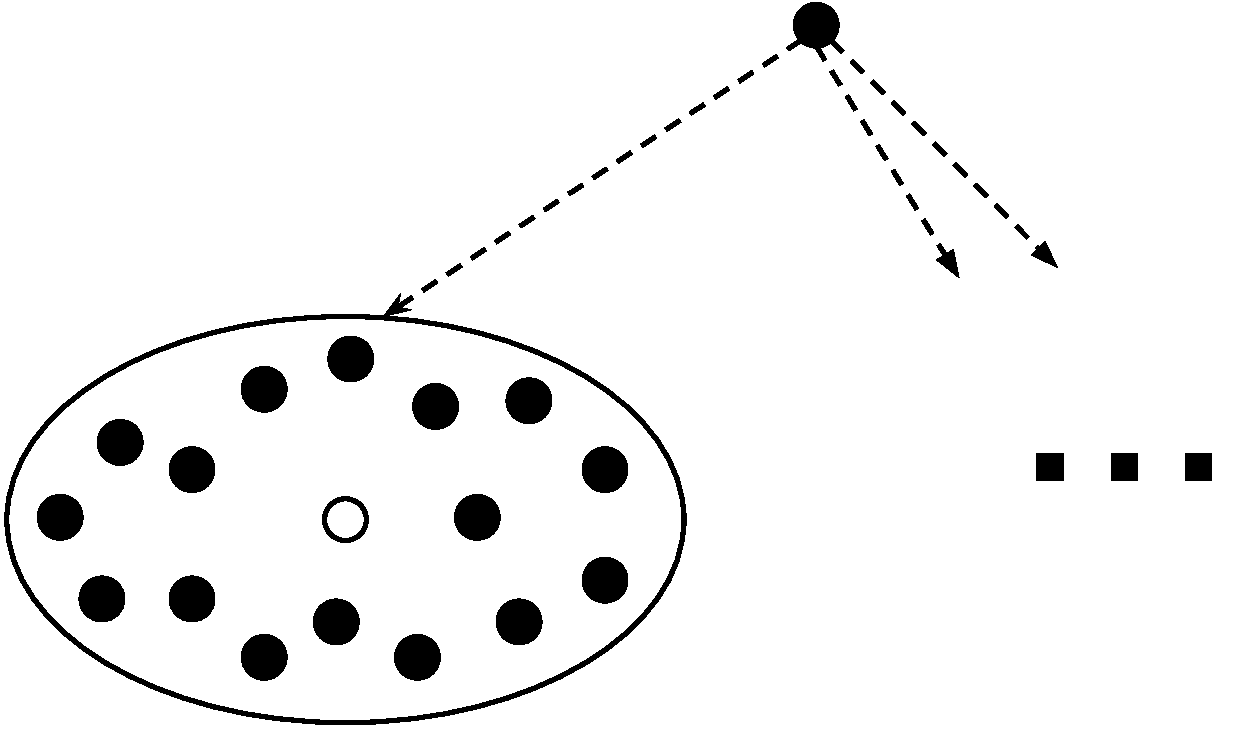
\includegraphics[scale=0.35]{PTree.pdf}
\caption{Graphical representation of $PTree$, $N$ Parallel work groups.}
\label{fig:PTree}
\end{figure}

\begin{figure}
\centering
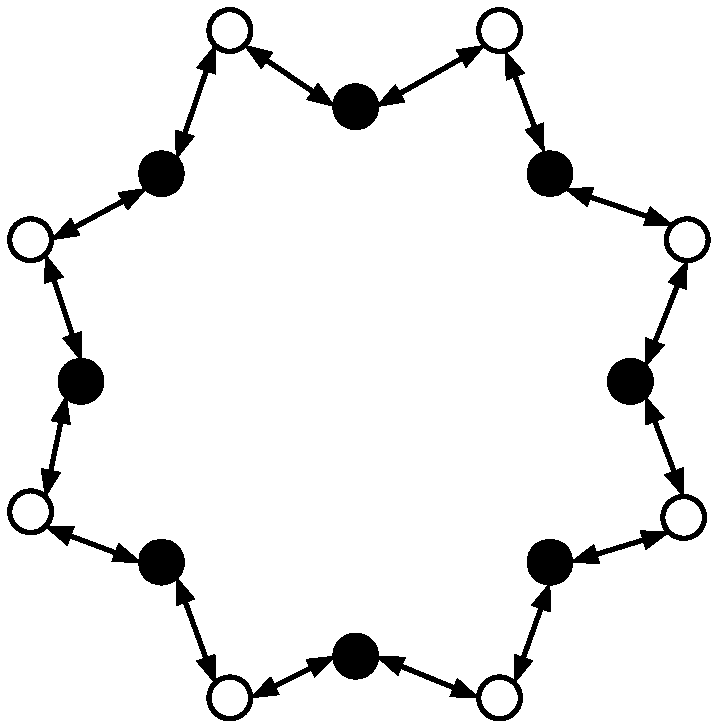
\includegraphics[scale=0.35]{PRing.pdf}
\caption{Graphical representation of $PRing$, full system predictable 
cooperation.}
\label{fig:PRing}
\end{figure}

\begin{figure}
\centering
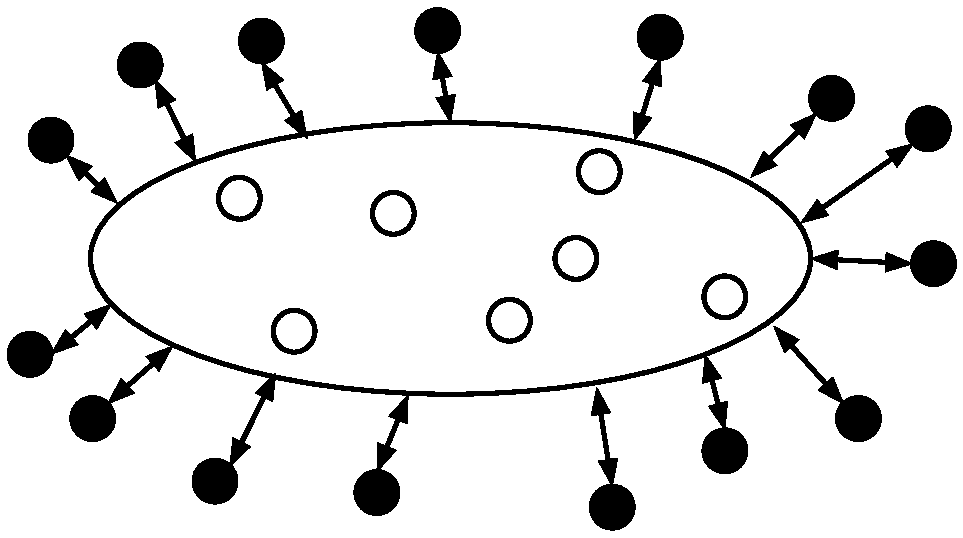
\includegraphics[scale=0.35]{ClusterComm.pdf}
\caption{Graphical representation of $ClusterComm$, $N$ processes to $M$ 
channels for unpredictable full system cooperation.}
\label{fig:ClusterComm}
\end{figure}

\begin{figure}
\centering
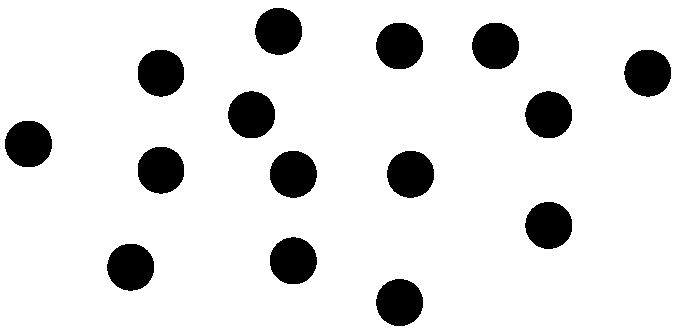
\includegraphics[scale=0.35]{ChugMachine.pdf}
\caption{Graphical representation of $ChugMachine$, $N$ worker processes 
without cooperation.}
\label{fig:}
\end{figure}

\begin{figure}
\centering
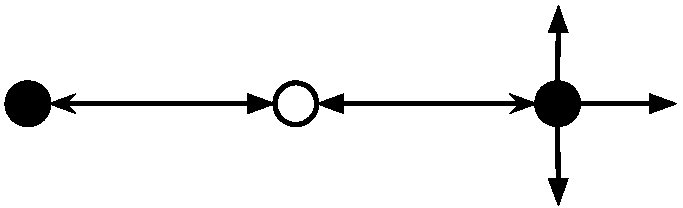
\includegraphics[scale=0.35]{UserInput.pdf}
\caption{Graphical representation of $UserInput$, single randomly hanging 
process.}
\label{fig:}
\end{figure}

\begin{figure}
\centering
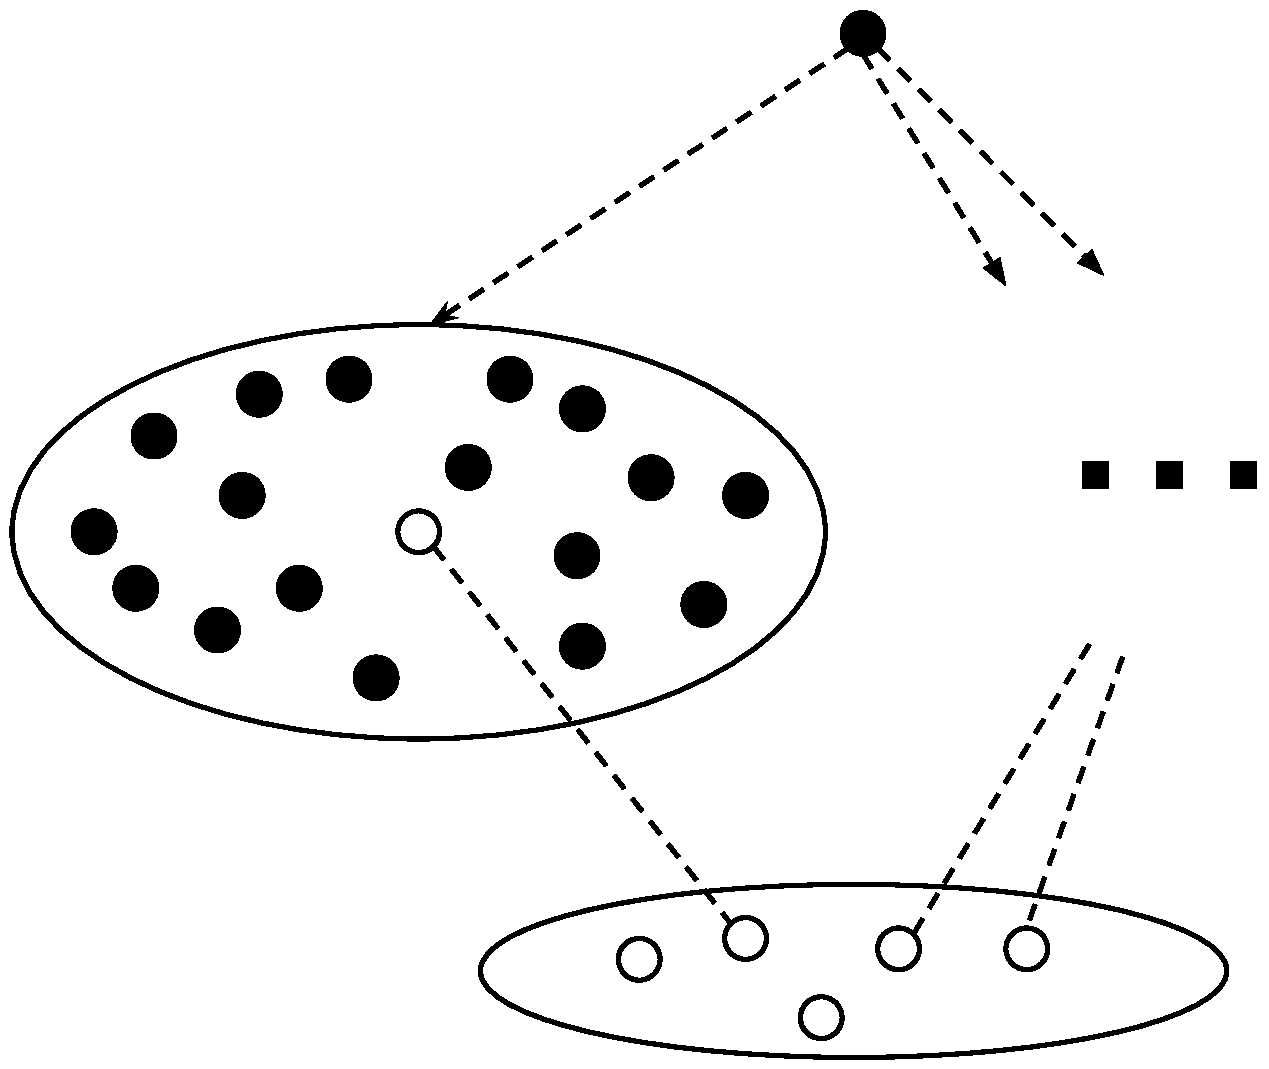
\includegraphics[scale=0.35]{JumpShip.pdf}
\caption{Graphical representation of $JumpShip$, $N$ Parallel phase shifting 
work groups.}
\label{fig:JumpShip}
\end{figure}





\section{Cooperativity Mechanics}\label{sec:cooperativity mechanics}

\subsection{Overview}\label{sec:cooperativity mechanics overview}
\subsection{Longevity-Based Batching}\label{sec:longevity based batching}
\subsection{Channel Pinning}\label{sec:channel pinning}
\subsection{Bipartite Graph Aided Shuffling}
    \label{sec:bipartite graph aided shuffling}



\chapter{Results and Discussion}
\index{Results and Discussion@\emph{Results and Discussion}}%
\label{chap:results}

\section{Evaluation}\label{sec:results-evaluation}

We begin our discussion by first stepping back and performing a meta-validation 
of the ErLam toolkit itself, before comparing the scheduling mechanisms amongst 
themselves. We ask:
\vspace{-3mm}\begin{itemize}
    \item How complex must our implementations be to create our test primitives? 
    \item For each scheduler, does our implementation work as expected, despite a minimalistic scheduler API?
    \item Does the channel implementation lend itself to scheduling improvements? If so, in what case?
\end{itemize}\vspace{-3mm}
These questions will evaluate ErLam, both as a language and runtime, but also as a 
simulator for scheduler experimentation, comparison, and evaluation. We attend to
these questions in order;
Section~\ref{sec:results-test-case-implementation} critiques the language as a 
medium for simulation design through the development of our test primitives.
Section~\ref{sec:results-evaluation-classical} discusses our evaluation of the
scheduler API using several of the testing primitives on the aforementioned 
classical schedulers. 
Then in section~\ref{sec:results-channel-implementations}, we discuss our findings 
regarding channel implementation differences and their subsequent effects on 
scheduling behavior.

\subsection{Test Case Implementation}\label{sec:results-test-case-implementation}

Our intentions when choosing our base language constructs were primarily focused on 
simplifying the base language. This minimalism we hoped would remove any noise 
which may be caused by the implementation details. We hoped to make, for lack of a better
term, a concurrent functional assembly language. As such, there was some concern
as to the level of ease we would be able to implement our testing primitives.

We start with a critique of the first implemented test case: $ChugMachine_N$. It
soon became apparent that we would need to standardize on a successive spawning
method for producing several of the same process at once. Rather than modifying
our $spawn$ expression we decided to implement this as a fuction in the language
as it was. The reasoning behind this was to keep consistent the effects of 
spawning a process into a process queue. If we allowed the process to produce $N$
processes at once, the lag caused by the runtime to produce them would be 
more noticable.

\begin{figure}
    \centering
{\footnotesize
\begin{BVerbatim}[commandchars=\\\{\}]
merge = \textbf{fun} a.(\textbf{let} x = \textbf{newchan} \textbf{in}
               \textbf{let} _ = (\textbf{spawn} \textbf{fun} _.(\textbf{swap} x (a nil))) \textbf{in}
               \textbf{fun} b.(\textbf{let} y = \textbf{newchan} \textbf{in} 
                      \textbf{let} _ = (\textbf{spawn} \textbf{fun} _.(\textbf{spawn} y (b nil))) \textbf{in}
                      \textbf{fun} m.(m (\textbf{swap} x nil) (\textbf{swap} y nil))))
// ...
(omega \textbf{fun} f,n.(\textbf{if} (leq n \textit{1}) 
                   (worker_t nil) 
                   (merge \textbf{fun} _.(f f (dec n)) worker_t ignore)) 
             N)
\end{BVerbatim}
}
    \caption{Our implementation for a map-reduce style fork-branch, and it's 
    subsequent standardized usage.}
    \label{fig:merge-code}
\end{figure}

We settled on the $merge$ function (figure~\ref{fig:merge-code}), along with a 
standard method of invoking it. Our $omega$ function would enable recursion, 
for us to use one branch of the $merge$ call to create a left-loaded binary
tree. This would keep a consistent behavior despite a bias towards the initial 
processes. Note that a work-stealing or global-queue scheduler would gain
access to the most recent processes sooner (and would thusly get a chance to
reduce sooner). 

Also as a side effect of our decision, there is a channel for every process which
immediately blocks. This has the added effect of giving us the ability to track when 
processes terminate, as the long-term blocked channels will start closing. For
example, figure~\ref{fig:fibonacci-channel-demo}, gives an example parallel
Fibonacci program written in this style and it's subsequent channel graph. This
is reminiscent of a map-reduce style approach, and the language lends itself
to it. Note on the channel graph, a dark line indicates a channel which 
becomes blocked until the point at which it becomes unblocked. 

\begin{SaveVerbatim}[commandchars=\\\{\}]{FibCode}
(omega \textbf{fun} f,m.(
    \textbf{if} (leq m 1) 
       m
       (merge \textbf{fun} _.(f f (sub m 1))
              \textbf{fun} _.(f f (sub m 2))
              add)) \textit{8})
\end{SaveVerbatim}
\begin{figure}[h!]

\subfigure{
    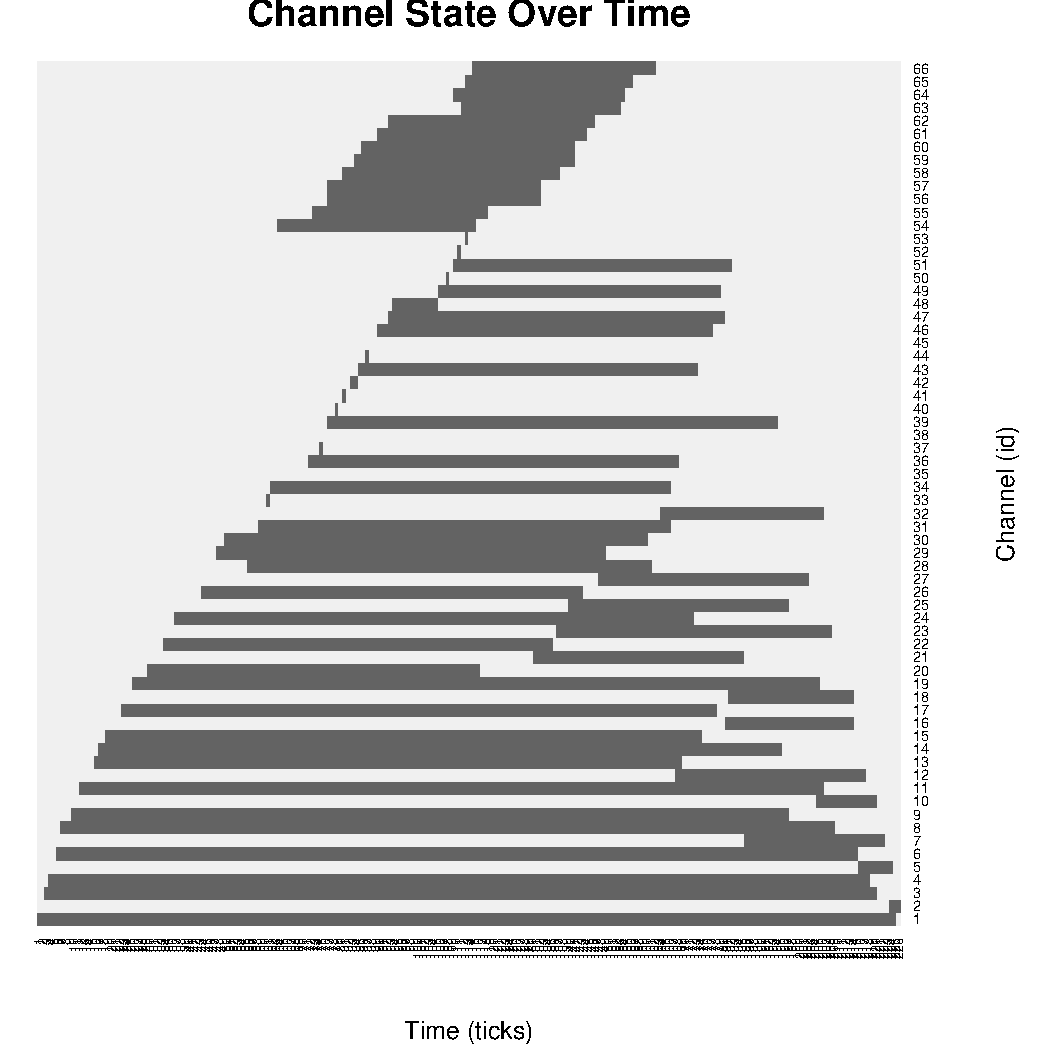
\includegraphics[scale=0.40]{fibonacci-channel-demo.pdf}
    \label{fig:fibonacci-channel-demo-chart}
}%
\subfigure{
    \centering
    \raisebox{20mm}{\footnotesize \BUseVerbatim{FibCode} }
\label{fig:fibonacci-channel-demo-code}
}
    \caption{Parallel Fibonacci implementation and a potential channel graph.}
    \label{fig:fibonacci-channel-demo}
\end{figure}

You may also note that the chart gives an indication as to the size of the time
quantum selected for the application's execution. The order in which a channel
becomes blocked, and it's order in the processes execution give that hint. The
large block of channels at the top of the graph indicate the last batch of 
spawned processes got time on the cpu before the one's which spawned it, as the
scheduler which evaluated the spawn ran out of reductions for that process. 
These observations will become useful for later scheduler critiques.

\subsection{Scheduler API}\label{sec:results-evaluation-classical}

The ErLam Scheduler API was minimally constructed around the single-step 
scheduling semantics presented earlier in figure~\ref{fig:scheduler-step}.
We were motivated by the simplicity of the description and thus the ability
to bring some formalism to the implementations. That being said, we would still
require the option to observe practical statistics such as runtime overhead 
during our scheduler comparisons. 

\begin{figure}[h!]
    \subfigure[Tick disparity, or the average time between scheduler ticks per 
    LPU, per Task run. Typical ranges tend to spike in groups, which show 
    consistency based on scheduler implementation, rather than OS intervention.]{
        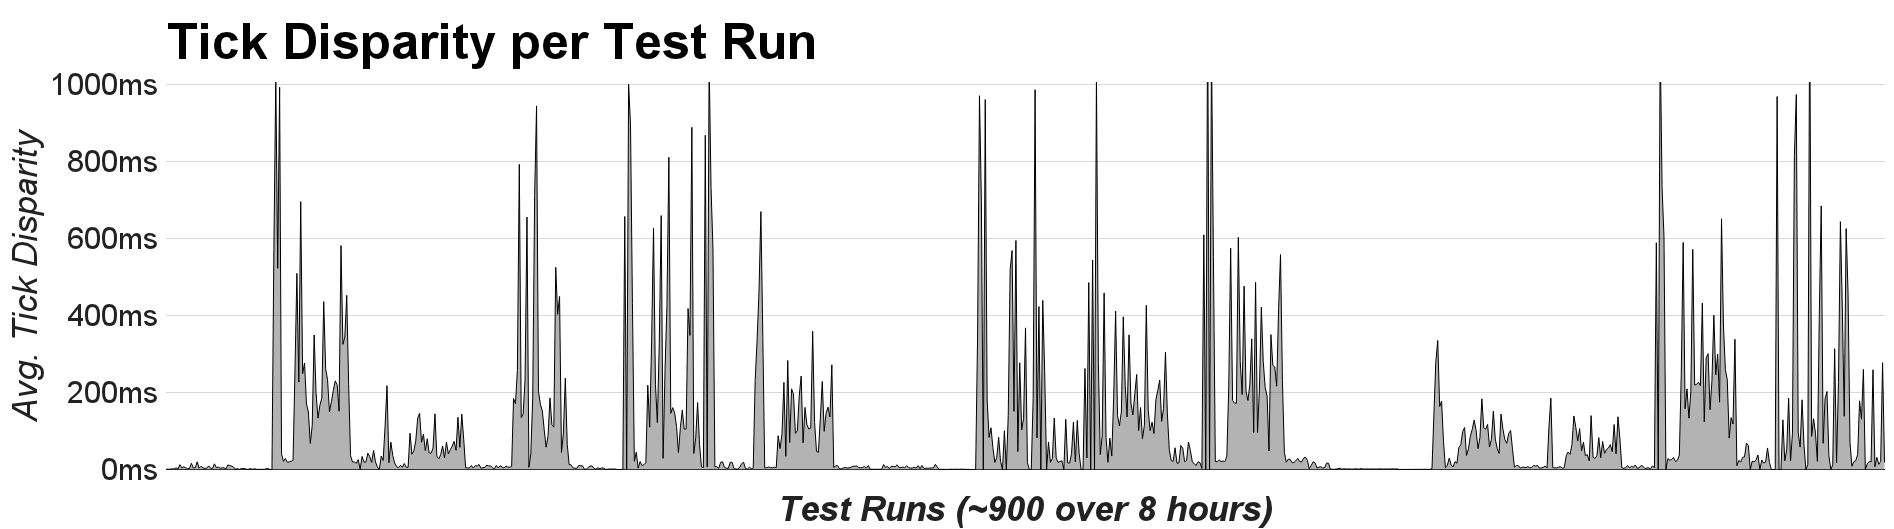
\includegraphics[width=\textwidth]{tick-disparity.png}
        \label{fig:tick-disparity}
    }
    \subfigure[Tick disparity consistently matches up with increased computation, 
    which is indicitive of inter-scheduler communication requirements.]{
        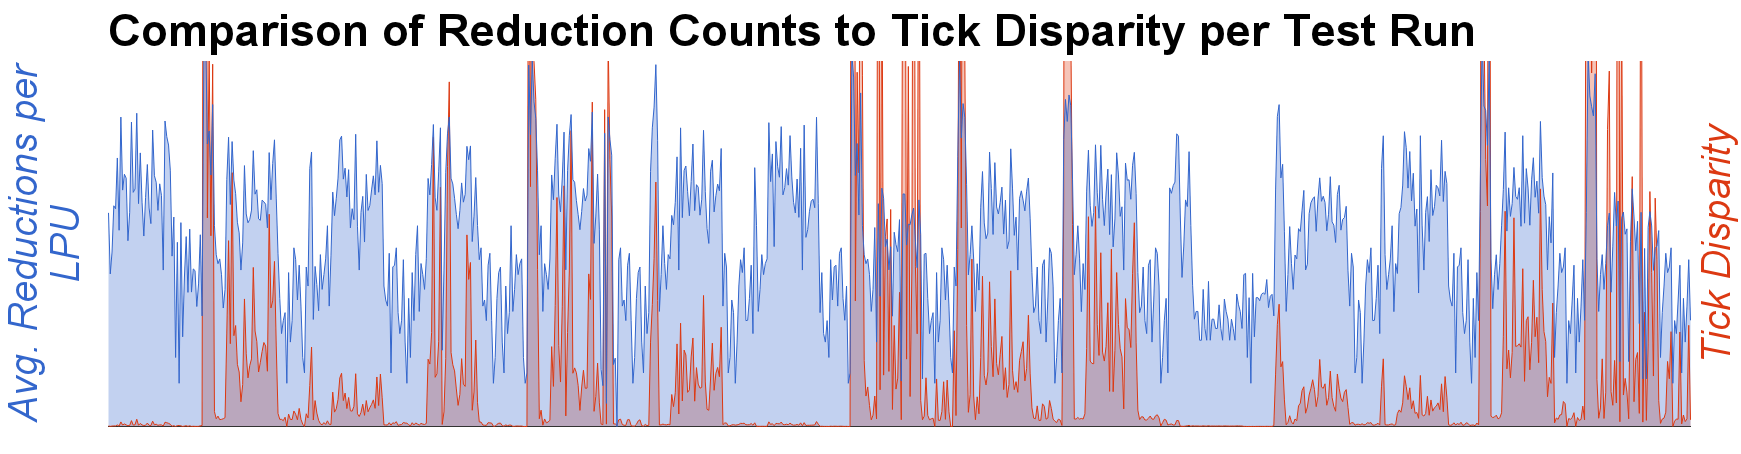
\includegraphics[width=\textwidth]{tick-disparity-to-reductions.png}
        \label{fig:tick-disparity-match}
    }
    \caption{Tick Disparity over nearly $900$ tests.}
\end{figure}

However,
wne of the concerns early on, and as described in section~\ref{sec:runtime log reports}, 
was that the LPUs could greatly differ in the number of ticks they are able to 
provide their process queue. This could be caused by the OS preempting the 
ErLam scheduling thread to execute something else. However, from our tests, we
found these gaps to be minimal and mainly caused by the scheduling implementation
itself. 

Figure~\ref{fig:tick-disparity} shows the average time between ticks averaged over
the LPUs for a large subsection of the tests we ran. We call this average time 
between ticks per LPU the Tick Disparity of the test. From the figure, we notice
obvious clustering, and figure~\ref{fig:tick-disparity-match} leads us to believe this
is primarily caused by spikes in reduction counts. A scheduler chugging on 
processes the entire time, must wait until preemption in-order to handle any 
inter-scheduler communication, as in the case of work-stealing schedulers. Thus,
for our purposes, all talk of tick-disparity could be considered a discussion of
scheduler overhead. As such, comparative analysis of scheduler implementation 
overhead from test case execution would still be a valid comparison with our
design.

Further, to validate that our scheduler implementations functioned as expected 
after translation was another concern. We gave the example of the CML 
Dual-Queue translation ($STDQ$) previously in section~\ref{sec:example the cml scheduler}.
We will now examine it's execution and compare it to $STRR$, a single queue naive
scheduler to confirm our understanding.

The key differences we would expect to see in a comparison would be that the CML
prefers to, and attempts to run the interactive processes first. It would push
all computational processes onto the secondary queue, only promoting them when 
the need arises. To observe this property, we compose the $UserInput_{(T,C)}$ 
test with $ChugMachine_N$ to create an interactivity test primitive 
$Interactivity_{(N,M)}$ (figure~\ref{fig:interactivity-code}). The primitive
launches $ChugMachine_N$ and $M$ instances of $UserInput_{(5,10)}$ (the values
of which were arbitrarily chosen so as to execute for long enough to collect
coherent data). We then subsequently ran this primitive with $STRR$ and $STDQ$
using multiple values for $N$ and $M$. Table~\ref{tab:interativity8-16-strr-stdq}
compares an instance of this test set: $Interactivity_{(8,16)}$.

\begin{table}[!p]
    \begin{tabular}{@{}ccc}
$Interactivity_{(8,16)}$ & \textbf{$STRR$}       & \textbf{$STDQ$}       \\ \cline{2-3} 
\multicolumn{1}{c|}{\rotatebox{90}{\textbf{Channel State over Time}}} & 
    \multicolumn{1}{l|}{\includegraphics[scale=0.32]{tests/interactivity/single/pg_0001.pdf}} & 
    \multicolumn{1}{l|}{\includegraphics[scale=0.32]{tests/interactivity/cml/pg_0001.pdf}} \\ \cline{2-3} 
    \multicolumn{1}{@{}c|}{\rotatebox{90}{\textbf{Communication Density}}}   & 
    \multicolumn{1}{l|}{\includegraphics[scale=0.32]{tests/interactivity/single/pg_0002.pdf}} & 
    \multicolumn{1}{l|}{\includegraphics[scale=0.32]{tests/interactivity/cml/pg_0002.pdf}} \\ \cline{2-3} 
\multicolumn{1}{c|}{\rotatebox{90}{\textbf{Reduction Density}}}       & 
    \multicolumn{1}{l|}{\includegraphics[scale=0.32]{tests/interactivity/single/pg_0003.pdf}} & 
    \multicolumn{1}{l|}{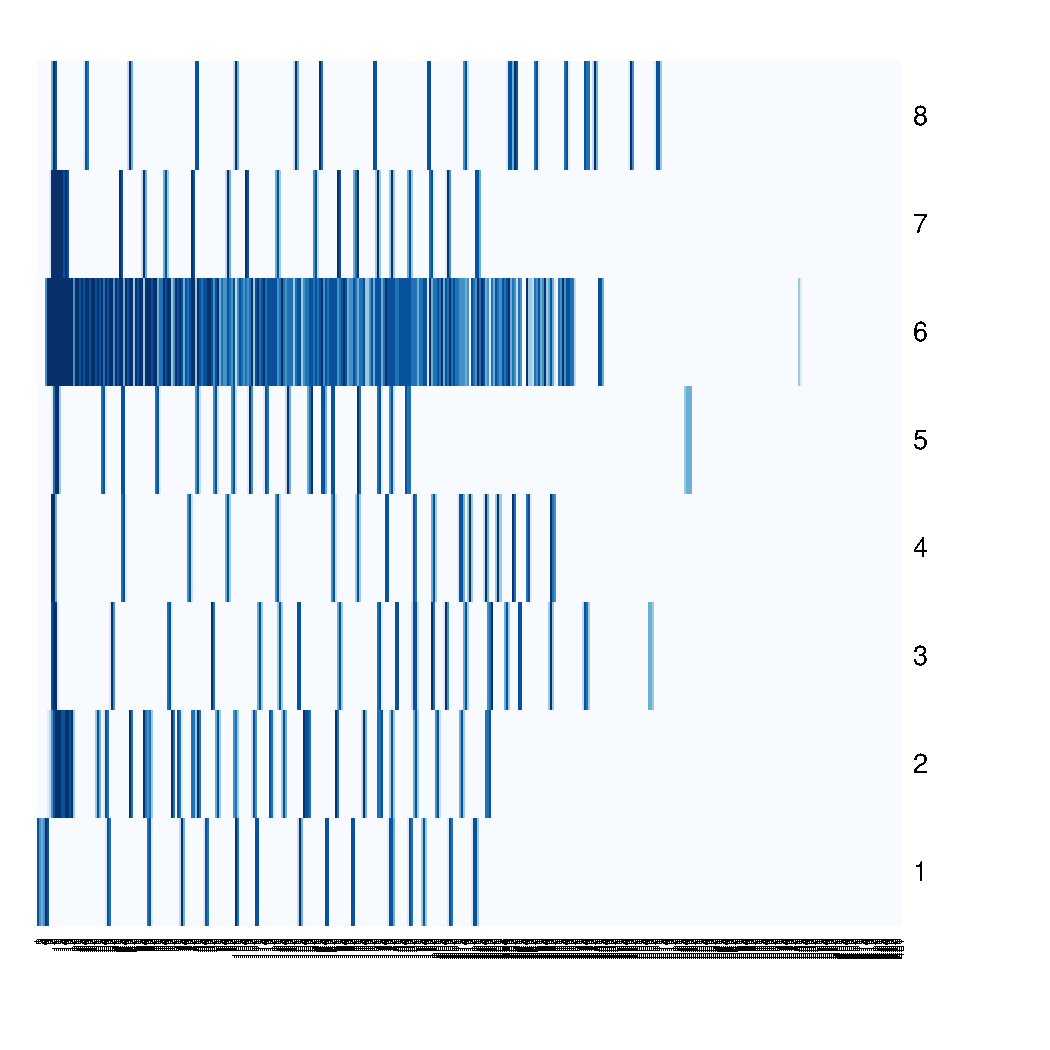
\includegraphics[scale=0.32]{tests/interactivity/cml/pg_0004.pdf}} \\ \cline{2-3} 
\end{tabular}
    \caption{Comparison of $STRR$ and $STDQ$ using Channel State, Reduction and Communication Densities.}
    \label{tab:interativity8-16-strr-stdq}
\end{table}

The Reduction Density graphs explain everything we need to know. The darkened portions
at the beginning of the chart indicate that the $STRR$ scheduler has no regard for the
interactive processes, whereas the $STDQ$ scheduler remains spread out. This seems to be
on the opposite if we were to consult the Communication Density charts though. It would appear
here that $STRR$ is getting more frequent communication, and $STDQ$ condenses all 
synchronizations to the end. This is however an issue of verbiage as Interactivity
does not correlate to Communication Density. By this we mean, $STRR$ is indeed allowing 
communication to happen evenly due to a round-robin schedule, but it is not attending to
spontanious events (\ie~responses back from $hang$). $STDQ$ on the otherhand pushes all 
inter-process communication backwards as it waits to respond to the $hang$ing processes.

We see this effect more clearly once we compare with the Channel State charts. In $STRR$
we see an even regard for all processes. The tapering of the channel blocks at the 
beginning of the graph is consistent with our understanding of the $merge$-based
successive spawning. However, $STDQ$ is completely different, and all $UserInput_{(T,C)}$
processes seem to be pushed to the beginning of the execution pool. This is infact due
to another difference between the execution styles of the two schedulers. $STDQ$ replaces
the currently running process with the child process it spawned, enqueuing the parent.
We therefore can confirm our understanding, in this case, that the scheduler is reacting
to the test primitives as expected.

The work-stealing mechanic is another instance for interesting comparison. We've built
two of the cooperativity-conscious schedulers we discuss on top of the $MTRRWS$-$*$ 
process queue implementation. It is this unified queue implementation which allows 
us to toggle between the two implementations. With $MTRRWS$-$SQ$, the process queue
will respond to function calls from schedulers for other LPUs, it will perform a
quick dequeue from the bottom only blocking the host LPU from accessing the queue
for a minimal amount of time. With $MTRRWS$-$IS$, the process queue goes untouched
by other LPUs, instead the scheduler on the LPU itself will receive the messages
and respond during periods inbetween process operations.

To compare these, we would expect to see minor differences in the processes scheduler 
state as we could expect $MTRRWS$-$IS$ to wait longer for responses from their theif
messages. But otherwise we would like to make sure the saturation of the cores are 
as identical as possible. In other words, if either method is unable to saturate the 
cores effectually, then it would not be worth further testing (or there is an issue 
with the implementation). 

However, work-stealing schedulers work best if there is a constant probability of 
loosing a process by completion. Our test primitives, as they stand, do not account for
application phases in terms of process quantity. Thus, to effectively examine these
stealing mechanisms, we substitute process loss via completion with process loss via 
channel absorption. Thus, table~\ref{tab:ptree9-10-5-wsis-wssq} gives a comparison of the 
two work-stealing techniques in terms of scheduler state over time and the process 
queue length with a run of $PTree_{(9,10)}$ with channel absorption turned on.

\begin{table}[!p]
    \begin{tabular}{@{}ccc}
$PTree_{(9,10)}$ & \textbf{$MTRRWS$-$IS$}       & \textbf{$MTRRWS$-$SQ$}       \\ \cline{2-3} 
\multicolumn{1}{c|}{\rotatebox{90}{\textbf{Scheduler State}}} & 
    \multicolumn{1}{l|}{\includegraphics[scale=0.32]{tests/ptree/wsis/pg_0005.pdf}} & 
    \multicolumn{1}{l|}{\includegraphics[scale=0.32]{tests/ptree/wssq/pg_0005.pdf}} \\ \cline{2-3} 
\multicolumn{1}{c|}{\rotatebox{90}{\textbf{Process Queue Length}}}   & 
    \multicolumn{1}{l|}{\includegraphics[scale=0.32]{tests/ptree/wsis/pg_0003.pdf}} & 
    \multicolumn{1}{l|}{\includegraphics[scale=0.32]{tests/ptree/wssq/pg_0003.pdf}} \\ \cline{2-3} 
\end{tabular}
    \caption{Comparison of $MTRRWS$-$IS$ and $MTRRWS$-$SQ$ using Scheduler State and Queue Size.}
    \label{tab:ptree9-10-5-wsis-wssq}
\end{table}


Upon review of this comparison, our initial assumptions are validated. The process queue
length looks extremely similar. The LPU which owns the initial process maintains the 
largest queue, where all others work steal a single process and work on it. Any gains in
queue size for these LPUs are via channel absorption, but this can not compare with the
initial spawns. We note here that an obvious introduction of smarter work-balancing
would be critical for a realistic or even practically useful scheduler. However, for our
purposes of verifying the work-stealing mechanism, this is sufficient.

The scheduler state comparison is however, in this instance, not consistent with all
the original assumptions. Namely, $MTRRWS$-$IS$ seems not stay in waiting mode as long
as $MTRRWS$-$SQ$ does. However, we can pose two possible reasons for this reaction:
there is an obvious scaling bias introduced by squeezing over $11000$ ticks into the same length
of space as $SQ$ does with $8000$. Alternatively, the scheduling reduction quantum for 
this execution was $20$ and all processes chug for only $5$ max, this allows the 
scheduler more opportunity to tend to inter-process communication at a detriment to
the shared-queue implementation due to higher chance of blocked queue access.

\subsection{Channel Implementations}\label{sec:results-channel-implementations}

The above graphs (\eg~table~\ref{tab:interativity8-16-strr-stdq}, and 
table~\ref{tab:ptree9-10-5-wsis-wssq}) were generated, using the CML-like Process 
Absorption channels. We would like to now breifly visualize how a blocking channel
may effect the scheduling of an application.

\todo[inline]{Give example of two runs with the same test/scheduler but with ca and cb.}


\section{Cooperativity Mechanics}\label{sec:results-evaluation-feedback}

We now turn to the discussion of cooperativity-conscious scheduling.
Using our classical scheduler results as a base line we can evaluate 
the feedback schedulers independently. This will give an indication of what
may warrant further investigation, and testing. However, there are three 
questions which are of immediate interest:
\vspace{-3mm}\begin{itemize}
    \item Are there instances where the stealing mechanism matters?
    \item When does being cooperativity-conscious lead to better schedules?
    \item Does the overhead of feedback systems outweigh the benefits?
\end{itemize}






\subsection{Longevity-Based Batching}\label{sec:results-longbatcher}
\subsection{Channel Pinning}\label{sec:results-channelpinner}
\subsection{Bipartite-Graph Aided Shuffling}\label{sec:results-smartsort}

\section{A Comment on Swap Channels}\label{sec:results-swap-channels}

Swap channels provided a number of benefits on the side of the language 
designer. They reduce the complexity of channel implementation, and as shown, 
they lend themselves to a number of possible designs. We demonstrated just two 
possible implementations, the Blocking and Absorption channels. As such, the 
concept of a swap channel as a language primitive is extremely attractive. 
However, swapping poses some problems for realistic applications which we would
now like to discuss.

\begin{figure}
\centering
\inputminted[frame=lines,fontsize=\footnotesize]{csharp}{code/badclustercomm.els}
\caption{A naive but ineffectual $ClusterComm_{(N,M)}$ implementation.} 
\label{fig:bad-clustercomm}
\end{figure}

First, a swap channel does not lend itself to a level of fairness that would be
expected by a programmer. We lead with our implementation of 
$ClusterComm_{(N,M)}$ as example, which due to being on top of swap channels, 
was made to be much more enigmatic. Figure~\ref{fig:bad-clustercomm} gives an
example implementation of $ClusterComm_{(N,M)}$. Note the third parameter to
the application, which denotes the number of time's each of the $N$ processes
should communicate. The system therefore blocks until all processes synchronize
$X$ times before quiting.

Due to this, we must pose several restrictions on the possible values of $N$ and
$M$. Namely, $N$ must be an even number, since all processes would need to have a 
partner to swap with, and $M$ must be no greater than $\lfloor N/2 \rfloor$, any
more and it would be possible for a process to hang indefinitely.

However, these two restrictions are not enough to guarantee the process terminates.
In fact, most runs of this application, with any value of $N > 2$ would most 
likely hang forever. This is due to the bias our program creates when spawning
processes, as well as the type of fairness the swap channel semantics provides.

First, our bias we introduce is merely because we cannot batch spawn a set of
processes at the same time. As such we will spawn one process at a time which
may get a chance to run before all others. As such the first several processes
may reach their synchronization limit before we are even done spawning the rest
of the processes. Due to this, we may have a case where all but $M$ processes
have completed, and thus all channels are blocked indefinitely.

Secondly, the channel semantics have no inherent preference for unseen 
or new processes. The scheduler may easily get in a loop of running the same
subset of processes repeatedly, this would have the same effect as the above
even if we were able to solve the bias problem. As such, this is inherently an
issue with the capabilities of swap channels. 

Thus, the best we can do for $ClusterComm_{(N,M)}$, is to run until at least 
$N-M$ processes have met their quota. Note this approach is only acceptable 
under Symmetric message passing constructs. In asymmetrical, even if there was
a guarantee of an equal number of senders and receivers, all senders could be
blocked on one channel while all receivers could be blocked on another. 

But this issue points to another problem with swap channels, insofar as they do
not lend themselves to being primitives at all. Due to this fairness issue, a 
language with swap channels would be unable to build the asymmetrical constructs
most user's would like. As such, they have been useful merely for simulation 
purposes.

However, for further simulation of cooperativity, it may be adventagous to also 
consider the directionality of communication. The recognition of consumer and 
producer processes may lend itself to further gains as the recognition of 
communication and computation bound processes did. This is not to say all gains
in utilizing pure synchronization have been obtained. 

\chapter{Conclusion and Future Work}
\index{Conclusion and Future Work@\emph{Conclusion and Future Work}}%
\label{chap:conclusions}

\section{Utility of the ErLam Toolkit}\label{sec:conclusions-erlam}

To test our scheduling mechanisms, the ErLam Toolkit provided a powerful framework
for their implementation and execution observation. The testing primitives provided
provide a concise way to reference common behavior and subsequently compare 
executions. The logging system was also precise enough to allow for further 
statistical comparison between multiple runs of the same test case. This allowed 
for easier fine-tuning as well as general algorithm debugging.

\section{Effectiveness of Cooperativity as a Metric}
\label{sec:conclusions-cooperativity}

Our original goal was to show several potentially adventagious mechanisms 
schedulers could use to take advantage of process cooperativity. We believe that 
we were able to validate most of our hypotheses and show that cooperativity can
be a powerful metric by which to govern a scheduler. With analysis of multiple 
test cases including boundary and common conditions, we proved the practicality of
these mechanisms as well. Ultimately we were able to open more avenues of possible
research in this field that we hope to explore further.

\section{Future Work}\label{sec:future-work}

There are a number of appealing avenues of improvement for the ErLam Toolkit. The
report generation mechanism could be extended and tied into the logging system a 
bit more  closely. For example, the implementation of a real-time viewer would be an 
interesting extension. Also, there are obviously a larger number of metrics which may lead
to better cooperativity classifications as well. It may be more fruitful, for 
example, to keep track of communication partners rather than channel names. 
The core language is also an appealing simulation implementation language, as such, a 
larger library of testing primitives would benefit the language designer community 
greatly. Furthermore, a complete catalog of parameterized executions would also aid 
in analysis and scheduler comparison.

In terms of cooperativity as a feedback metric, it would be interesting to further
tweak the three cooperativity-conscious schedulers already implemented. Perhaps 
composing the scheduler mechanics themselves may lead to a more robust algorithm.
For example, the combination of the Batching and Channel Pinning may lead to a better
work stealing mechanism as batches now belong to channels. Alternatively the ability
to sort batches might speed up the sorting process. It would also reduce the search
space for finding related processes when it came time to resort. However, in short, 
the future of cooperativity as a feedback metric looks promising.



%\include{chapter-instructions}
%\include{chapter-howtouse}
%\include{chapter-makingbib}
%\include{chapter-tables+figs}
%\include{chapter-math}


%%%%%%%%%%%%%%%%%%%%%%%%%%%%%%%%%%%%%%%%%%%%%%%%%%%%%%%%%%%%%%%%%%%%%%
% Appendix/Appendices                                                %
%%%%%%%%%%%%%%%%%%%%%%%%%%%%%%%%%%%%%%%%%%%%%%%%%%%%%%%%%%%%%%%%%%%%%%
%
% If you have only one appendix, use the command \appendix instead
% of \appendices.
%
%\appendices
%\index{Appendices@\emph{Appendices}}%

%\chapter{Lerma's Appendix}
\index{Appendix!Lerma's Appendix@\emph{Lerma's Appendix}}%
The source \LaTeX{} file for this document is no longer quoted in
its entirety in the output document. A \LaTeX{} file can 
include its own source by using the command
\cn{verbatiminput\{\cn{jobname}\}}.



%%%%%%%%%%%%%%%%%%%%%%%%%%%%%%%%%%%%%%%%%%%
\chapter{My Appendix \#2}
\index{Appendix!My Appendix \#2@\emph{My Appendix \#2}}%
\section{The First Section}
This is the first section.
This is the second appendix.

\section{The Second Section}
This is the second section of the second appendix.

\subsection{The First Subsection of the Second Section}
This is the first subsection of the second section of the second appendix.

\subsection{The Second Subsection of the Second Section}
This is the second subsection of the second section of the second appendix.

\subsubsection{The First Subsubsection of the Second Subsection of
		the Second Section}
This is the first subsubsection of the second subsection of the
second section of the second appendix.

\subsubsection{The Second Subsubsection of the Second Subsection
		of the Second Section}
This is the second subsubsection of the second subsection of the
second section of the second appendix.


%%%%%%%%%%%%%%%%%%%%%%%%%%%%%%%%%%%%%%%%%%%
\chapter{My Appendix \#3}
\index{Appendix!My Appendix \#3@\emph{My Appendix \#3}}%

\section{The First Section}
This is the first section.
This is the third appendix.

\section{The Second Section}
This is the second section of the third appendix.





%%%%%%%%%%%%%%%%%%%%%%%%%%%%%%%%%%%%%%%%%%%%%%%%%%%%%%%%%%%%%%%%%%%%%%
% Generate the bibliography.                         %
%%%%%%%%%%%%%%%%%%%%%%%%%%%%%%%%%%%%%%%%%%%%%%%%%%%%%%%%%%%%%%%%%%%%%%
%                                    %
% NOTE: For master's theses and reports, NOTHING is permitted to     %
%   come between the bibliography and the vita. The command      %
%   to generate the index (if used) MUST be moved to before      %
%   this section.                            %
%                                    %
%
\nocite{*}      % This command causes all items in the           %
                % bibliographic database to be added to          %
                % the bibliography, even if they are not         %
                % explicitly cited in the text.              %
        %                            %
  % Here the bibliography           %
        % is inserted.                %

\index{Bibliography@\emph{Bibliography}}%
\bibliographystyle{plain}
\bibliography{thesis}
%%%%%%%%%%%%%%%%%%%%%%%%%%%%%%%%%%%%%%%%%%%%%%%%%%%%%%%%%%%%%%%%%%%%%%


%%%%%%%%%%%%%%%%%%%%%%%%%%%%%%%%%%%%%%%%%%%%%%%%%%%%%%%%%%%%%%%%%%%%%%
% Generate the index.                            %
%%%%%%%%%%%%%%%%%%%%%%%%%%%%%%%%%%%%%%%%%%%%%%%%%%%%%%%%%%%%%%%%%%%%%%
%                                    %
% NOTE: For master's theses and reports, NOTHING is permitted to     %
%   come between the bibliography and the vita. This section     %
%   to generate the index (if used) MUST be moved to before      %
%   the bibliography section.                    %
%                                    %
%\printindex%    % Include the index here. Comment out this line      %
%       % with a percent sign if you do not want an index.   %
%%%%%%%%%%%%%%%%%%%%%%%%%%%%%%%%%%%%%%%%%%%%%%%%%%%%%%%%%%%%%%%%%%%%%%


%%%%%%%%%%%%%%%%%%%%%%%%%%%%%%%%%%%%%%%%%%%%%%%%%%%%%%%%%%%%%%%%%%%%%%
% Vita page.                                 %
%%%%%%%%%%%%%%%%%%%%%%%%%%%%%%%%%%%%%%%%%%%%%%%%%%%%%%%%%%%%%%%%%%%%%%
\begin{vita}
\end{vita}
\end{document}
